%%%%%%%%%%%%%%%%%%%%%%%%%%%%%%%%%%%%
% TikZ - code:
% Schematic illustration of 
% of the Landau model
% Author: Sascha Fleer
%%%%%%%%%%%%%%%%%%%%%%%%%%%%%%%%%%%%

\documentclass[crop,tikz]{standalone}

\usetikzlibrary{decorations.pathreplacing}

\begin{document}
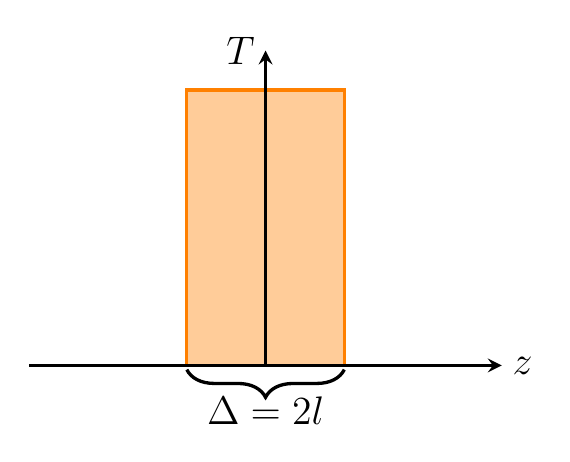
\begin{tikzpicture}[scale=1,>=stealth,font=\Large]
    \def\weg1{(2,0) -- (2,3.5) -- (4,3.5) -- (4,0)};    
    
    \fill[orange, opacity=0.4] \weg1;
    \draw[very thick, orange] \weg1;
    \draw [decorate,decoration={brace,amplitude=10pt,mirror},very thick,yshift=-1.5pt]
(2,0) -- (4,0) node [below,midway,yshift=-6pt]{$\Delta=2l$};

    \draw[very thick,<-] (3,4) node[left] {$T$} -- (3,0);
    \draw[very thick,<-]  (6,0) node[right] {$z$}  -- (0,0);
 \end{tikzpicture}
 \end{document}
